\documentclass{beamer}
%\usetheme{Copenhagen}
\usetheme{Madrid}
\title{Introduction to Kalman Filtering}
\subtitle{An Engineer's Perspective}
\author{Prof. x \and Someone}
\institute[SCUT] % (optional)
{
%	\inst{1}%
  School of Automation Science and Engineering\\
  South China University of Technology
	\and
%	\inst{2}%
%	Faculty of Chemistry\\
%	Very Famous University
}
\date{June 17, 2023}
\usepackage{mathtools}
\usepackage{color}
\usepackage{graphics}
\usepackage{hyperref}
\usepackage{listings}

\logo{
\includegraphics[height=0.6cm]{logo1}}
% Adapted from beamerinnerthemedfault.sty
% set the itemize item symbol as a diamond
\setbeamertemplate{itemizeitem}{\scriptsize$\diamond$}
% set the itemize subitem symbol as a triangle
\setbeamertemplate{itemize subitem}{\scriptsize$\blacktriangleright$}
% set the itemize subsubitem symbol as a circle with a dot
\setbeamertemplate{itemize subsubitem}{\scriptsize$\odot$}


\AtBeginSubsection[]
{
	\begin{frame}
		\frametitle{Table of Contents}
		\tableofcontents[currentsubsection]
	\end{frame}
}

\begin{document}

\begin{frame}
\titlepage
\end{frame}

\begin{frame}
\frametitle{Outline}
\tableofcontents
\end{frame}

\section{Introduction}

\subsection{History}

% test for \onslide
%\begin{frame}
%	\frametitle{List}
%	\begin{itemize}
%		\pause
%		\item Point A
%		\pause
%		\item Point B
%		\begin{itemize}
%			\pause
%			\item part 1
%			\pause
%			\item part 2
%		\end{itemize}
%		\pause
%		\item Point C
%		\pause
%		\item Point D
%	\end{itemize}
%\end{frame}

%\begin{frame}
%	\begin{align*}
%		\onslide<1->{a &= b \\}
%		\onslide<2->{b &= c \\}
%		\onslide<3>{\Rightarrow \quad 
%			a &= c}
%	\end{align*}
%\end{frame}


\begin{frame}
	\frametitle{Introduction to Kalman Filter}
	\begin{columns}
		\column{0.7\textwidth}
			\begin{itemize}
				\item Developed by Rudolf E. Kalman
					\begin{itemize}
						\item Born in 1930 in Hungary
						\item Education: B.S., M.S. from MIT; Ph.D. (1957) from Columbia
						\item Developed Kalman Filter in 1960-61
					\end{itemize}
				\item Filter: just a fancy word for an algorithm that takes an input (typically, a sensor signal) and calculates a function of that input
				\item Kalman Filter: an efficient, recursive filter that estimates the state of a dynamic system from a series of noisy measurements
			\end{itemize}
		\column{0.3\textwidth}
		\begin{figure}
			\centering
			% Requires \usepackage{graphicx}
			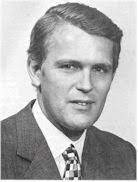
\includegraphics[width=2cm]{kalman.jpeg}\\
			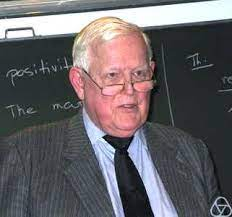
\includegraphics[width=2cm]{kalman21.jpeg}
		\end{figure}%
	\end{columns}
\end{frame}

\begin{frame}
	\frametitle{Introduction to Kalman Filter}
	Rudolf Kalman developed the Kalman Filter in the 1960’s. The
	filter was used to help control spacecraft navigation systems. It
	was even used in the NASA Apollo missions to the moon!
	\begin{figure}
			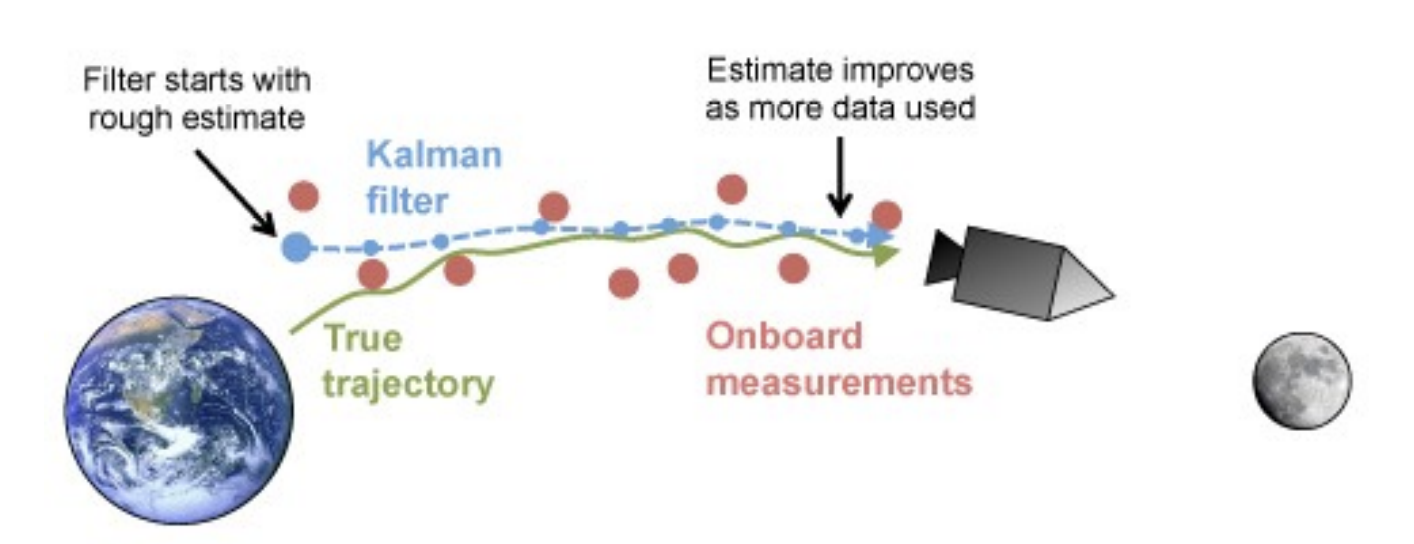
\includegraphics[width=3.5in]{aerospace.png}
		\end{figure}
\end{frame}

\begin{frame}
	\frametitle{What is a Kalman Filter used for?}
	Broadly, it’s useful for any type of tracking application, such as
	\begin{itemize}
		\item Tracking missiles
		\item Estimating position of aircraft
		\item Surveillance of highway traffic
		\item GPS-based motion estimation
		\item Economics applications (e.g., estimating demand for international reserves)
		\item Mobile robot localization!
	\end{itemize}
\end{frame}



%\begin{frame}
%	\frametitle{Bullet style in Beamer}
%%	\begin{itemize}
%%		\item Level 1
%%		\begin{itemize}
%%			\item Level 2
%%			\begin{itemize}
%%				\item Level 3
%%			\end{itemize}
%%		\end{itemize}
%%	\end{itemize}
%
%\begin{columns}
%	\column{0.5\textwidth}
%	\begin{itemize}
%		\item {
%			A $(t,n)$ threshold secret sharing scheme allows a dealer to split her secret $s$ into $n$ pieces (also called shares) and distribute them among $n$ parties. 
%		}
%		\item {
%			In a threshold scheme any $t$ or more than $t$ shareholders can reconstruct the secret. 
%		}
%	\end{itemize}
%	\column{0.5\textwidth}
%	\begin{figure}
%		\centering
%		% Requires \usepackage{graphicx}
%		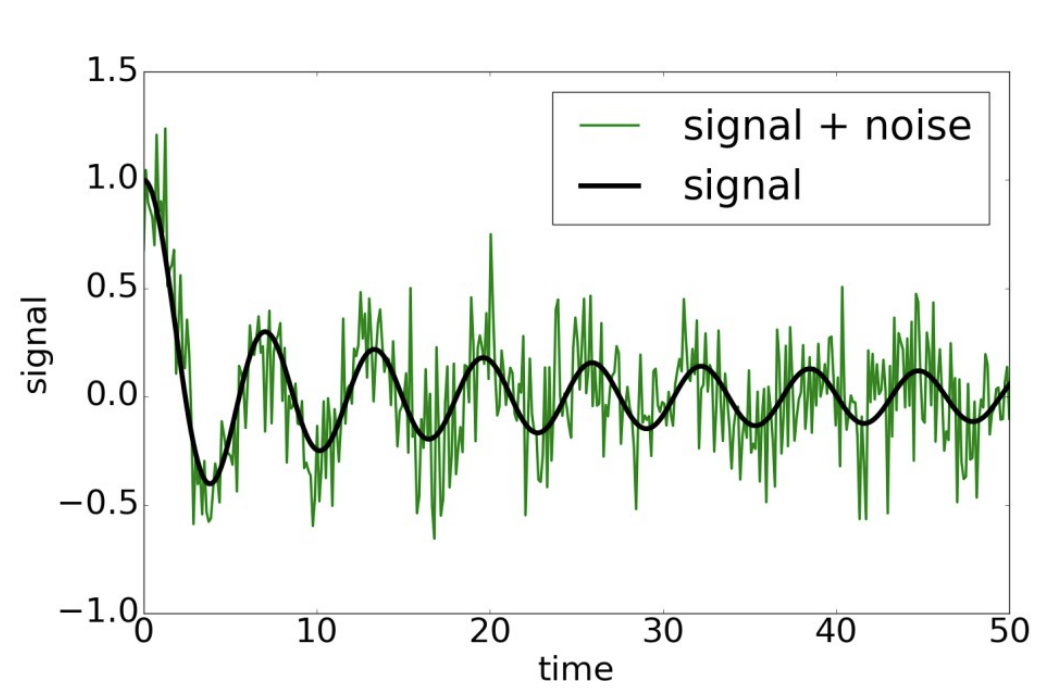
\includegraphics[width=3cm]{signal1.png}\\
%		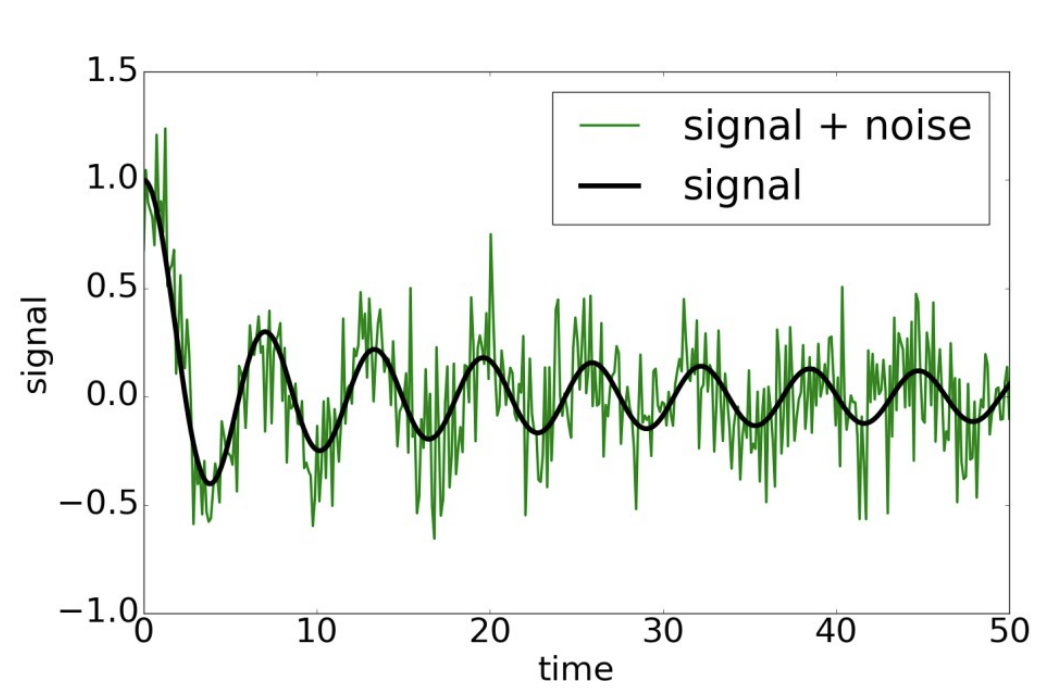
\includegraphics[width=3cm]{signal1.png}
%	\end{figure}%
%\end{columns}
%\end{frame}


%\begin{frame}
%	\frametitle{History of the Kalman Filter}
%	Developed around 1960 mainly by Rudolf E. Kalman.  It was originally designed for aerospace guidance applications, which is an extension
%	of the Wiener Filter to nonstationary (and usually discrete)
%	signals..  
%	A central problem in signal processing is filtering, finding a signal in noise
%	\begin{figure}
%		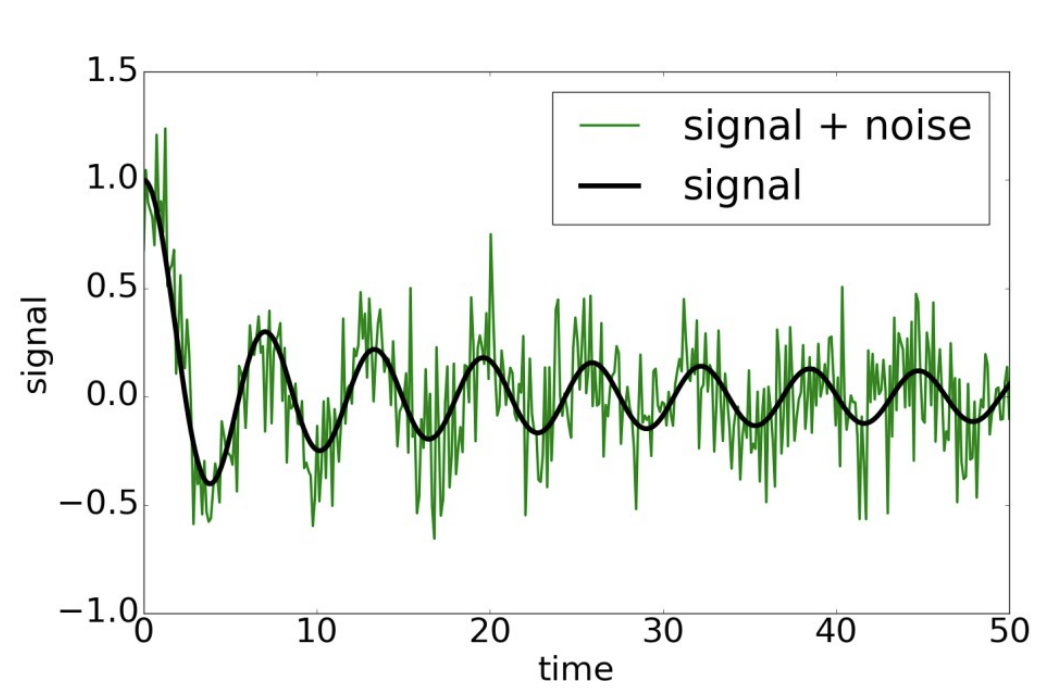
\includegraphics[width=2.5in]{signal1.png}
%	\end{figure}
%\end{frame}
%
%\begin{frame}
%	\frametitle{History of the Kalman Filter}
%	The	filter was used to help control spacecraft navigation systems. It
%	was even used in the NASA Apollo missions to the moon!
%	\begin{figure}
%		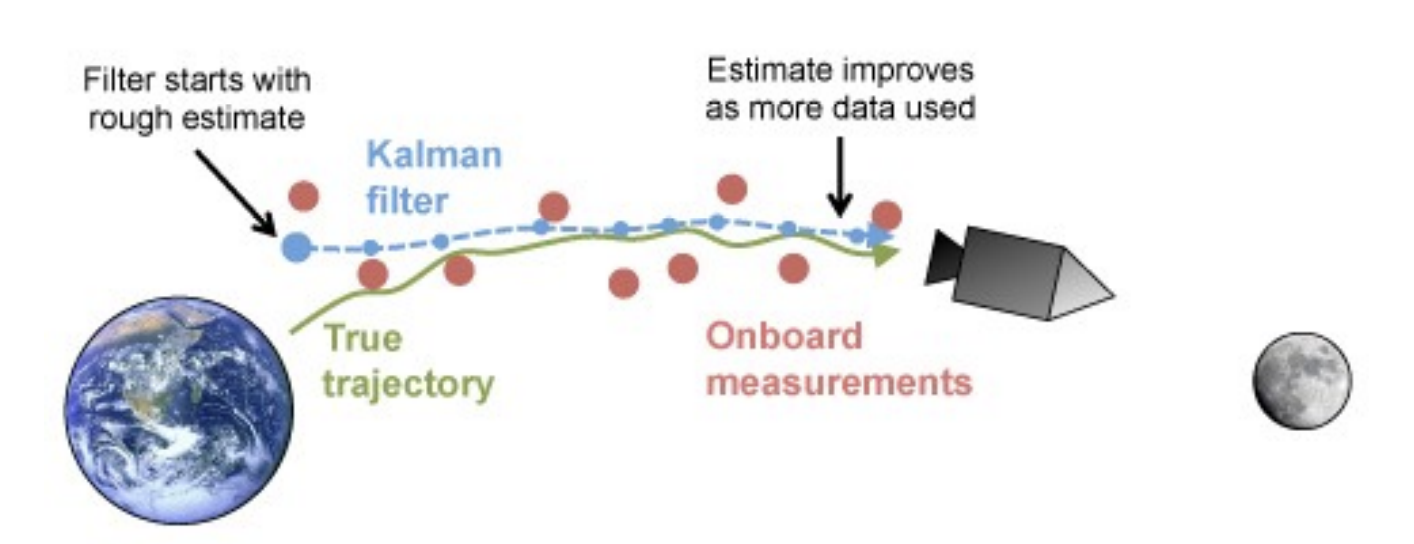
\includegraphics[width=2.5in]{aerospace.png}
%	\end{figure}
%\end{frame}

\subsection{Motivation}

%\begin{frame}
%	\begin{enumerate}
%		\item{bla}
%		\begin{enumerate}
%			\item{blubb}
%			\begin{enumerate}
%				\item{foo}
%			\end{enumerate}
%		\end{enumerate}
%	\end{enumerate}
%\end{frame}


\begin{frame}
\frametitle{Why Use Kalman Filters?}
\begin{columns}
	\column{0.6\textwidth}
		\begin{block}{Remark}
			A Kalman filter is an optimal estimation algorithm used to estimate states of a system from indirect and uncertain measurements.
		\end{block}
		Kalman filter is used when:
		
			\begin{itemize}
			\item  The variables of interest can only be measured indirectly. 
			\item Measurements are available from various sensors but might be subject to noise.
		\end{itemize}
		
		
		
	\column{0.4\textwidth}
		\begin{figure}
			\centering
			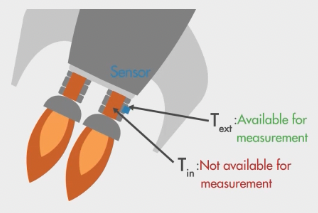
\includegraphics[width=4.7cm]{example1.png}
			\caption{Kalman filter used to estimate the internal temperature of a combustion chamber}
		\end{figure}
	\end{columns}
\end{frame}

\begin{frame}
	\frametitle{Why Use Kalman Filters?}
	\begin{figure}
		\centering
		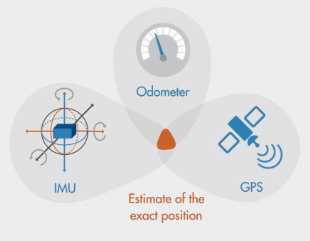
\includegraphics[width=5.5cm]{example2.png}
		\caption{Estimate the state of a system (e.g., the position of a car) by fusing measurements from multiple sources (e.g., an inertial measurement unit (IMU), an odometer, and a GPS receiver) in the presence of noisy measurements. }
	\end{figure}
	
\end{frame}

\section{Algorithm}
\subsection{State Observers}

\begin{frame}
	\frametitle{How to estimate the internal temperature of a jet engine?}
	\begin{itemize}
		\item  There isn't any feasible way of measuring the internal temperature $T_{in} $, since $T_{in} $  is too high.
		\item Place the sensor on a colder surface and measure the temperature there, which called external temperature $T_{ext} $.
		\item Available signals are fuel flow and external temperature measurements
	\end{itemize}
	\begin{figure}
		\centering
		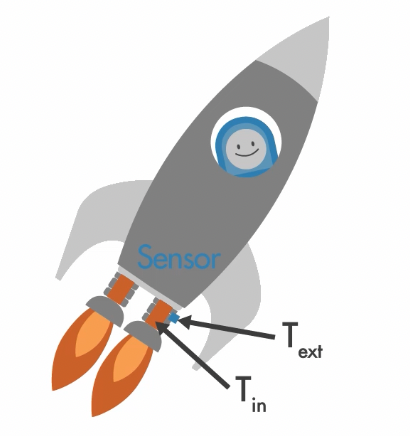
\includegraphics[width=3.5cm]{T_jet.png}
		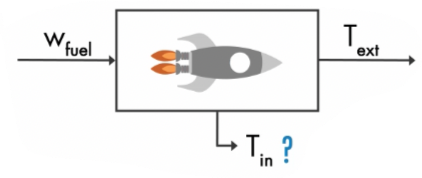
\includegraphics[width=4.5cm]{T_observer.png}
	\end{figure}
\end{frame}

\begin{frame}
	\frametitle{A possible solution}
	\begin{block}{Remark}
		If the state x is shown with a hat $\hat{x}$, then it is an estimated state. 
	\end{block}
Find a mathematical model of the temperature change and, given the known inputs, calculate the internal state of the system.
	\begin{columns}
		
		\column{0.3\textwidth}
			\begin{figure}
				\centering
				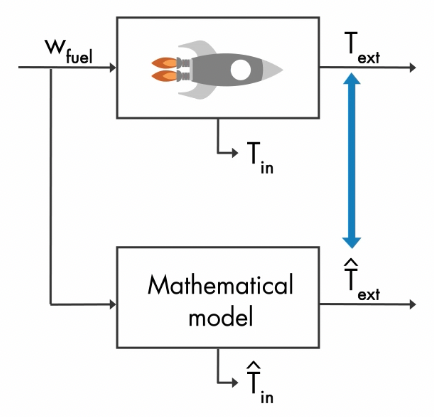
\includegraphics[width=3.5cm]{T_observer_solution.png}
			\end{figure}
		\column{0.7\textwidth}
		\begin{itemize}
			\item There are modeling errors
			\item The system is affected by uncertain factors
			\item A state estimator is required to estimate the internal state
		\end{itemize}
		\end{columns}
\end{frame}

\begin{frame}
	\frametitle{How a state estimator works?}
	\begin{itemize}
		\item  The goal is to match $\hat{T}_{ext}$ with the measured $T_{ext}$
		\item If $\hat{T}_{ext}=T_{ext}$, then the model will converge to the real system, and $\hat{T}_{in}$ will converge to its true value
		\item Minimize the difference between the estimated and measured external temperature
	\end{itemize}
	\begin{figure}
		\centering
		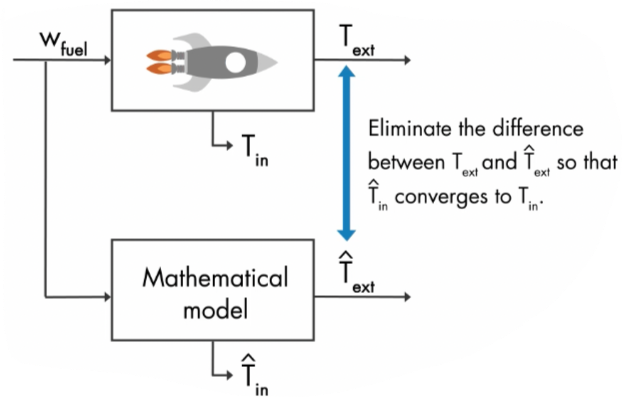
\includegraphics[width=6.2cm]{T_fbcontrol.png}
	\end{figure}
\end{frame}

\begin{frame}
	\frametitle{Introducing a Feedback Control System}
	{\color{red}{Question}}: How to choose the controller gain k such that the error between the measured and estimated external temperature is minimized optimally?
	\begin{figure}
		\centering
		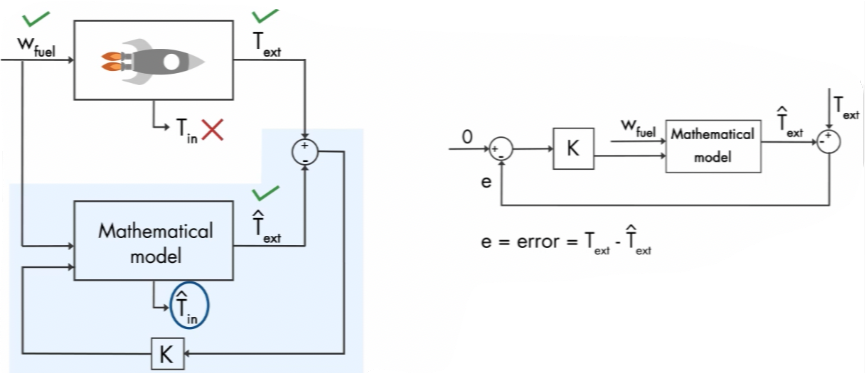
\includegraphics[width=11cm]{observer.png}
	\end{figure}
 
\end{frame}

\begin{frame}
	\frametitle{mathematical perspective}
	We can interpret the state observer mathematically as:
	\begin{figure}
		\centering
		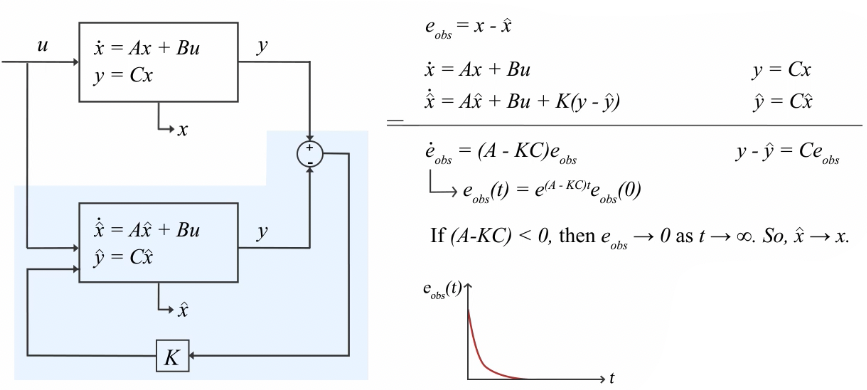
\includegraphics[width=11cm]{observer1.png}
	\end{figure}
\end{frame}

\begin{frame}
	\frametitle{mathematical perspective}
	\begin{itemize}
	    \item The significance of having a feedback loop around the observer is that we can control the decaying rate of the error function by selecting the controller gain k accordingly. 
	    
	    \item If there are some uncertainties in the mathematical model, you can't control how quickly the error will vanish.
	    
	    \item An optimal way of choosing the gain k is performed through the use of Kalman filters.
    \end{itemize}
\end{frame}


\subsection{Optimal State Estimator}

\begin{frame}
	\frametitle{Example of estimate the car's position}
	\begin{columns}
		\column{0.5\textwidth}
		Let's assume the car measures its position using GPS.
			\begin{itemize}
				\item The input to the car is a throttle. 
				\item The output that we're interested in is the car's position. 
				\item  For such a system, we would have multiple states. 
			\end{itemize}

		\column{0.5\textwidth}
			\begin{figure}
				\centering
				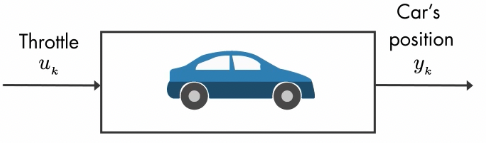
\includegraphics[width=5.3cm]{car_pos.png}\\
				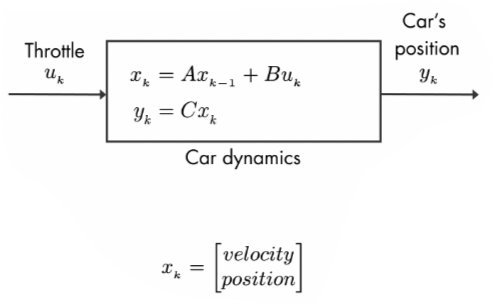
\includegraphics[width=5.4cm]{car_dynamic.png}
			\end{figure}
		
	\end{columns}
\end{frame}

\begin{frame}
	For simplicity, we take the speed of the car as input without loss of generality
	\begin{figure}
		\centering
		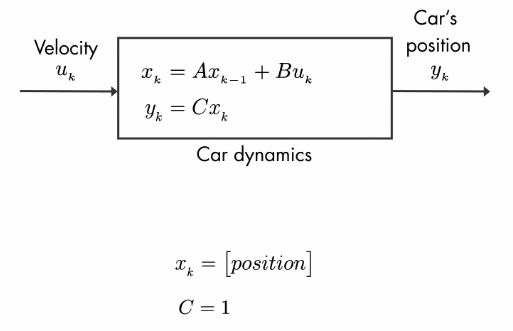
\includegraphics[width=6cm]{car_vel.png}
	\end{figure}
\end{frame}

\begin{frame}
	There is measurement noise  in the position measurements obtained using GPS.
	
	\begin{itemize}
		\item $v_k $ is assumed to be drawn from a Gaussian distribution with zero mean and covariance R.
		\item Similarly, the process noise $\omega_k $ is also random and assumes a Gaussian distribution with covariance Q. 
	\end{itemize}
	\begin{figure}
		\centering
		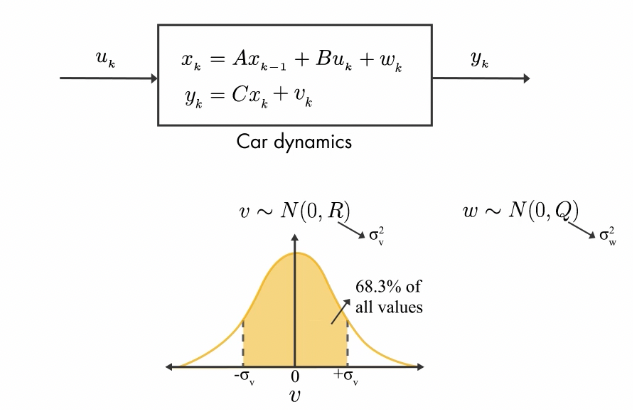
\includegraphics[width=7cm]{car_noise.png}
	\end{figure}
\end{frame}

\begin{frame}
	\frametitle{The role of the Kalman filter}
		\begin{itemize}
			\item Due to the presence of measurement noise, the measurements do not fully reflect the real position of the car.
			\item There is also uncertainty in the prediction of the car's position due to process noise.
		\end{itemize}
    This is where the Kalman filter comes into play:
	\begin{figure}
		\centering
		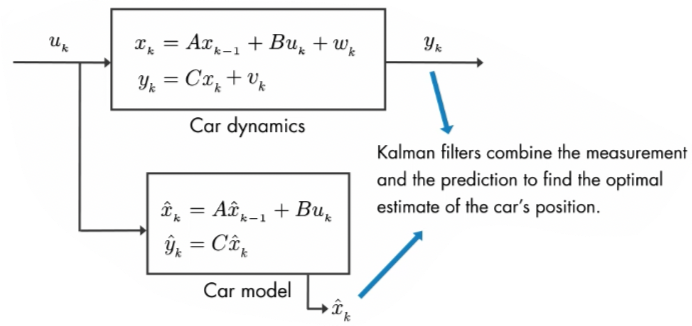
\includegraphics[width=8cm]{car_kf.png}
	\end{figure}
\end{frame}

\begin{frame}
	\frametitle{Probability Perspective}
	We can intuitively understand how the Kalman filter works with the help of the probability density function.
	\begin{figure}
		\centering
		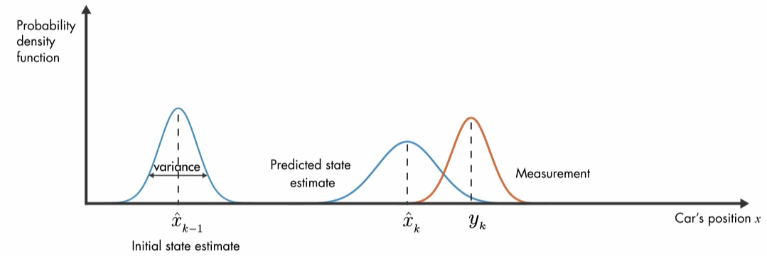
\includegraphics[width=11cm]{car_kf_relation.png}
	\end{figure}
\end{frame}

\begin{frame}
	\frametitle{Probability Perspective}
	 It turns out that the optimal way to estimate the car's position is by combining these two pieces of information. 
	 
	\begin{figure}
		\centering
		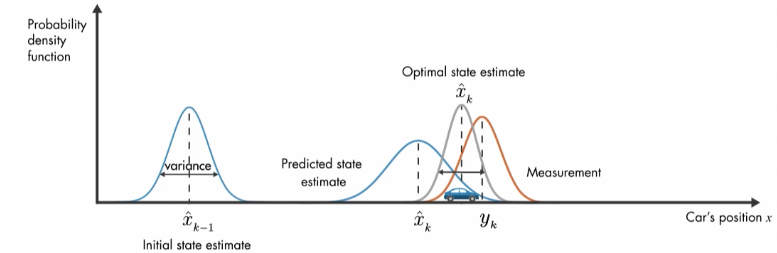
\includegraphics[width=11cm]{car_kf_relation1.png}
	\end{figure}
\end{frame}

\subsection{Kalman Filter Algorithm}

\begin{frame}
	\frametitle{Problem definition}
	Kalman filters are used to estimate states based on linear dynamical systems in state space format. As shown in the previous example:
	\begin{figure}
		\centering
			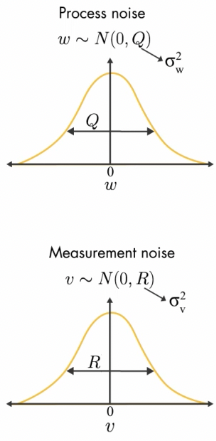
\includegraphics[width=2.6cm]{state_observer_of_previous1.png}
			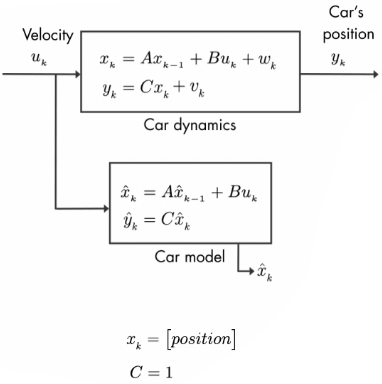
\includegraphics[width=4.7cm]{state_observer_of_previous.png}
	\end{figure}
\end{frame}

%\begin{frame}
%	\begin{figure}
%		\centering
%		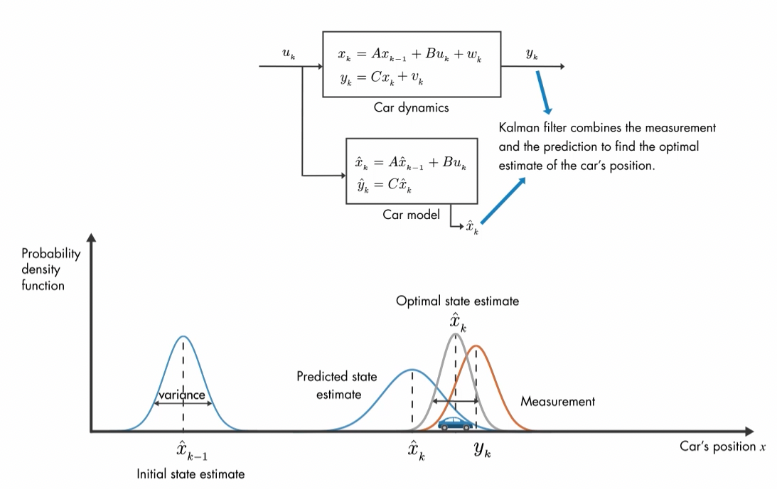
\includegraphics[width=11cm]{kf_back2.png}
%	\end{figure}
%\end{frame}

\begin{frame}
	\frametitle{Kalman filter}
	Now we directly give the expression of the optimal estimate given by the kalman filter:
	\begin{figure}
		\centering
		
\includegraphics[width=11.5cm]{kf_algorithm.png}\\
		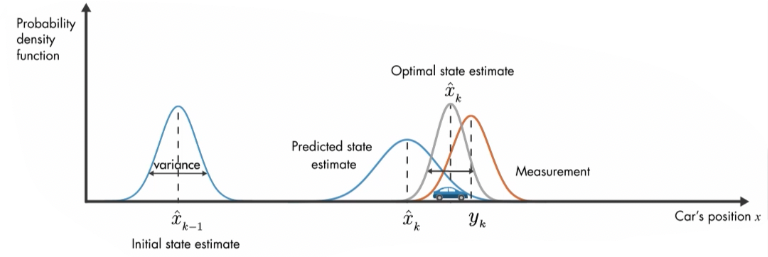
\includegraphics[width=11cm]{kf_algorithm1.png}
	\end{figure}

\end{frame}

\begin{frame}
	\frametitle{Kalman filter}
	It looks like the state observer equation discussed earlier. 
	\begin{figure}
		\centering
		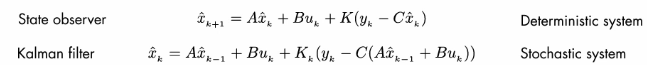
\includegraphics[width=10.5cm]{observer_kalman.png}
	\end{figure}
	\begin{block}{Remark}
		Actually, a Kalman filter is a type of state observer, but it is designed for stochastic systems. 
	\end{block}
\end{frame}

\begin{frame}
	\frametitle{Kalman filter}
	The first part predicts the current state by using state estimates from the previous timestep and the current input, called the a priori estimate.
	\begin{figure}
		\centering
		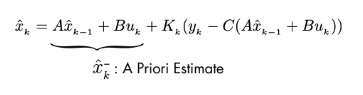
\includegraphics[width=6cm]{kf_back4.png}
	\end{figure}
	We can now rewrite the equation, and the second part of the equation uses the measurement and incorporate it into the prediction to update the a priori estimate.
	\begin{figure}
		\centering
		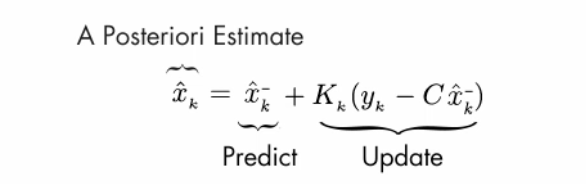
\includegraphics[width=5.4cm]{kf_back5.png}
	\end{figure}

\end{frame}

\begin{frame}
	\frametitle{Kalman filter}
	Kalman filter algorithm consists of two stages: prediction and update. 
	\begin{block}{Remark}
		Note that the terms “prediction” and “update” are often called “propagation” and “correction,” respectively, in different literature. 
	\end{block}
	The Kalman filter algorithm is summarized as follows:
	\begin{figure}
		\centering
		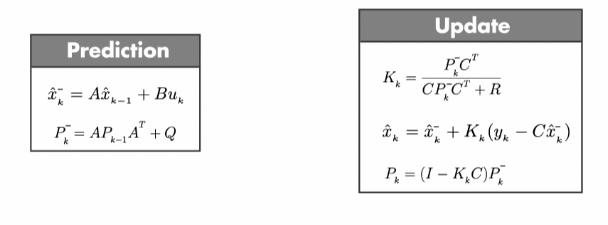
\includegraphics[width=8cm]{kf.png}
	\end{figure}
\end{frame}

\begin{frame}
	\frametitle{Kalman filter: Prediction}
	\begin{block}{Remark}
		The new term P is called state error covariance. It encrypts the error
		covariance that the filter thinks the estimate error has.
	\end{block}
	\begin{itemize}
		\item The system model is used to calculate the a priori state estimate:
	\end{itemize}
	\begin{figure}
		\centering
		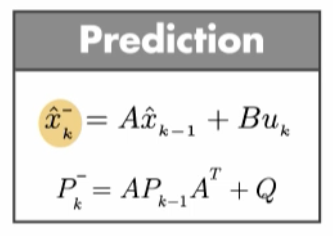
\includegraphics[width=2.2cm]{priori_state_estimate.png}
		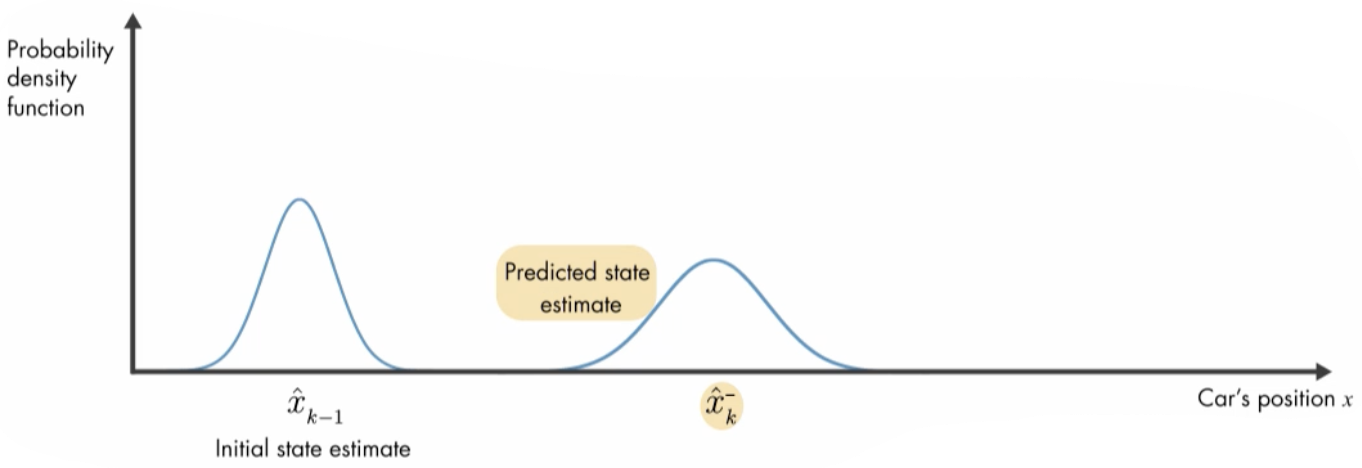
\includegraphics[width=8cm]{priori_state_estimate1.png}
	\end{figure}
\end{frame}

\begin{frame}
	\frametitle{Kalman filter: Prediction}
	and the error covariance $P^-_k $ .
	\begin{figure}
		\centering
		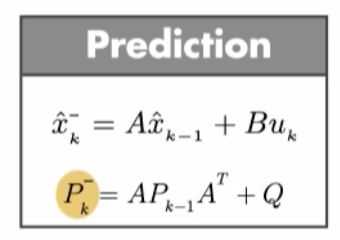
\includegraphics[width=2.3cm]{priori_error_cov.png}
		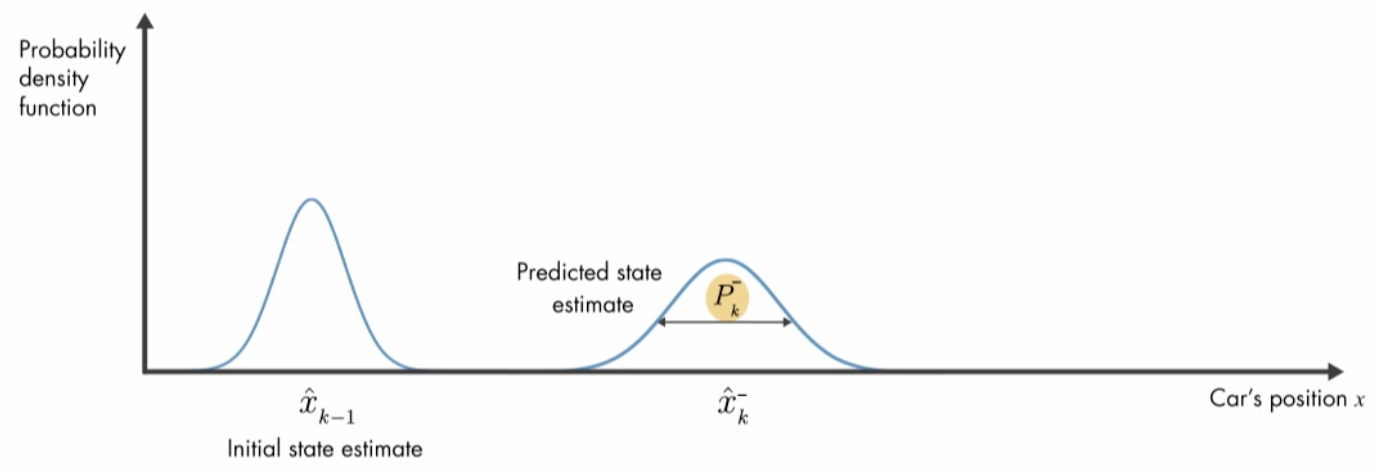
\includegraphics[width=8.2cm]{priori_error_cov1.png}
	\end{figure}
		
\end{frame}

\begin{frame}
	\frametitle{Kalman filter: Prediction}
	\begin{itemize}
		\item $P^-_k $ is the variance of the a priori estimate, and it can be thought of as a measure of uncertainty in the estimated state. This variance comes from the process noise and propagation of the uncertain $\hat{x}_{k-1} $ .
		\item At the very start of the algorithm, $\hat{x}_{k-1} $ and $P_{k-1} $ come from their initial estimates. 
	\end{itemize}
	\begin{figure}
		\centering
		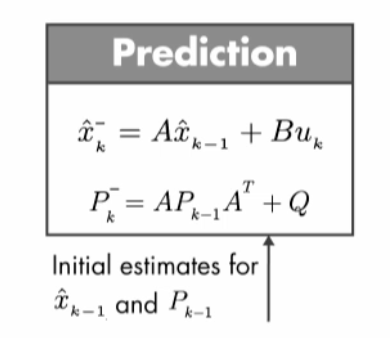
\includegraphics[width=3cm]{initial.png}
	\end{figure}
\end{frame}

\begin{frame}
	\frametitle{Kalman filter: Update}
	 
	\begin{block}{Remark}
		The derivation of $K_k $ and $P_k $ can refer to \href{https://en.wikipedia.org/wiki/Kalman_filter}{\color{blue}{\underline{wikipedia}}}.
	\end{block}
	\begin{itemize}
		\item The second step of the algorithm uses the a priori estimates calculated in the prediction step and updates them to find the a posteriori estimates of the state and error covariance.
		\item The Kalman gain is calculated such that it minimizes the a posteriori error covariance $P_k $. 
	\end{itemize}
	\begin{figure}
		\centering
		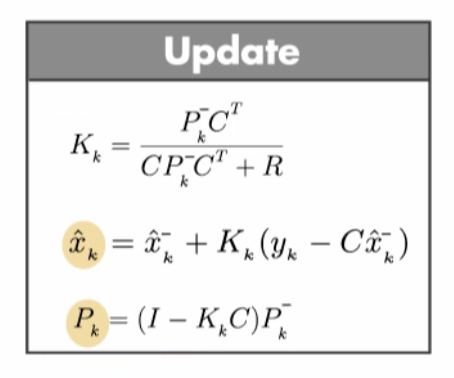
\includegraphics[width=3cm]{update.png}
	\end{figure}
	
	
\end{frame}

\begin{frame}
	\frametitle{Kalman gain}
	Let this bar represent the calculation of  $\hat{x}_{k} $. By weighing the correction term, the Kalman gain determines how heavily the measurements and the a priori estimates contributes to the calculation of $\hat{x}_{k} $.
	\begin{figure}
		\centering
		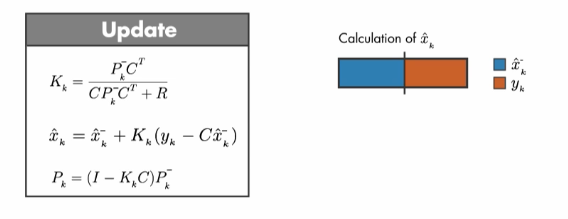
\includegraphics[width=7.5cm]{kf_gain.png}
	\end{figure}
\end{frame}

\begin{frame}
	\frametitle{Kalman gain}
	\begin{block}{Remark}
		\begin{itemize}
			\item  	If the measurement noise is small, the measurements is trusted more and contributes to the calculation of $\hat{x}_{k} $ more than the a priori state estimate does. 
			\item In the opposite case, where the error in the a priori estimate is small, the a priori estimate is trusted more. And the computation of $\hat{x}_{k} $ mostly comes from this estimate.
		\end{itemize}
	\end{block}
We can also show this mathematically by looking at two extreme cases: $R \to 0 $ and $P^-_k  \to 0 $.
\end{frame}
\begin{frame}
	If $R \to 0 $, we found that the a posteriori estimate is equal to the measurement.
	\begin{figure}
		\centering
		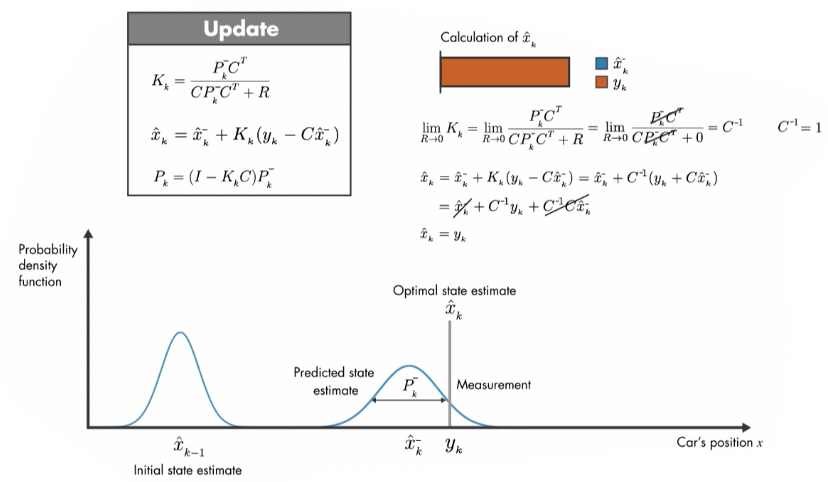
\includegraphics[width=10cm]{kf_gain_R0.png}
	\end{figure}
\end{frame}

\begin{frame}
	If $P^-_k  \to 0 $, the computation of $\hat{x}_{k} $ comes from the a priori state estimates.
	\begin{figure}
		\centering
		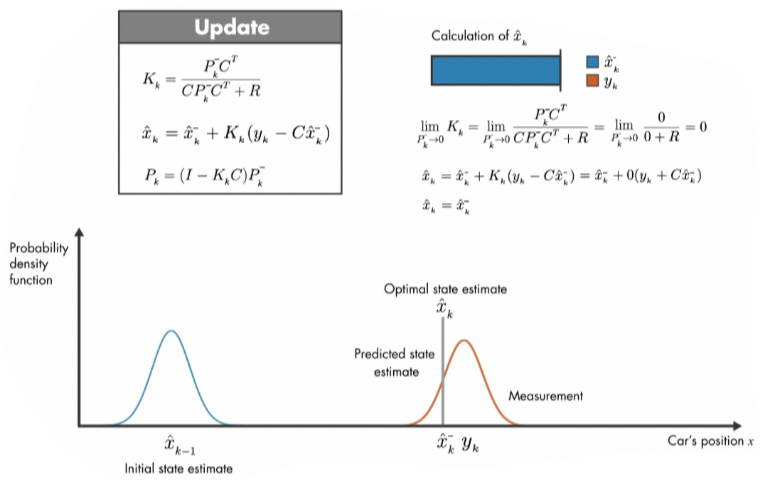
\includegraphics[width=9.7cm]{kf_gain_P0.png}
	\end{figure}
\end{frame}

\begin{frame}
	\frametitle{Kalman filter}
	\begin{block}{Remark}
		Notice that to estimate the current state, the algorithm only needs the estimated state and error covariance matrix from the previous timestep and the current measurement.
	\end{block}
	Kalman filter recursive:
	\begin{figure}
		\centering
		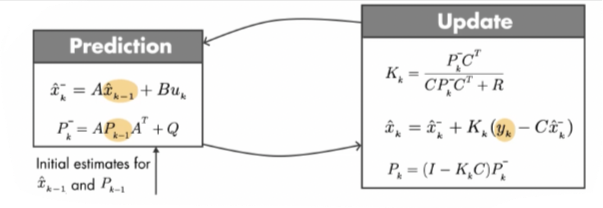
\includegraphics[width=8cm]{kf_loop.png}
	\end{figure}
\end{frame}

\begin{frame}
	\frametitle{Kalman filter: Sensor fusion}
	\begin{block}{Remark}
		Note that the Kalman filter is also referred as a sensor fusion algorithm. 
	\end{block}
If using additional sensor such as an IMU.  the dimensions of y, C, and K matrices will change as shown here
	\begin{figure}
		\centering
		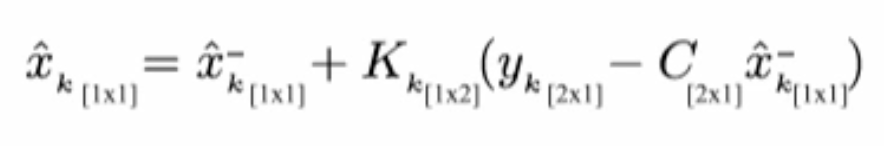
\includegraphics[width=5cm]{kf_multi_sensor.png}
	\end{figure}
\end{frame}

\begin{frame}
	\frametitle{Kalman filter: Sensor fusion}
	 In probability perspective, we'll be multiplying three probability density functions together to find the optimal estimate of the car's position.
	\begin{figure}
		\centering
		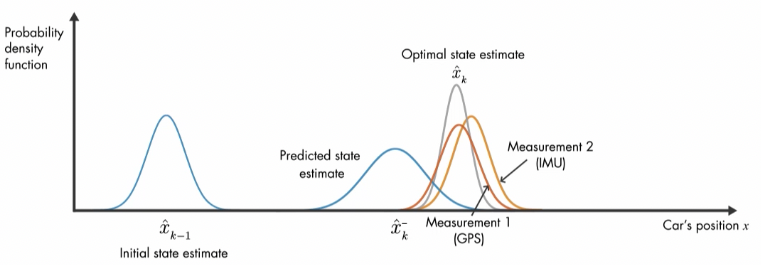
\includegraphics[width=11cm]{kf_multi_sensor1.png}
	\end{figure}
\end{frame}

\subsection{Extended Kalman filters}
\begin{frame}
	In a general system, either the state transition function, or the measurement function or both may be nonlinear. 
	\begin{figure}
		\centering
		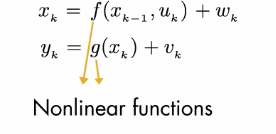
\includegraphics[width=4.5cm]{ekf2.png}
	\end{figure}
	For all these cases, we need to use a nonlinear state estimator instead of a Kalman filter, as Kalman filters are only defined for linear systems: 
	\begin{figure}
		\centering
		
\includegraphics[width=7.5cm]{ekf1.png}
	\end{figure}
\end{frame}

\begin{frame}
	 In this case, we can implement an extended Kalman filter (EKF), which linearizes the nonlinear function around the mean of the current state estimate. 
	\begin{figure}
		\centering
		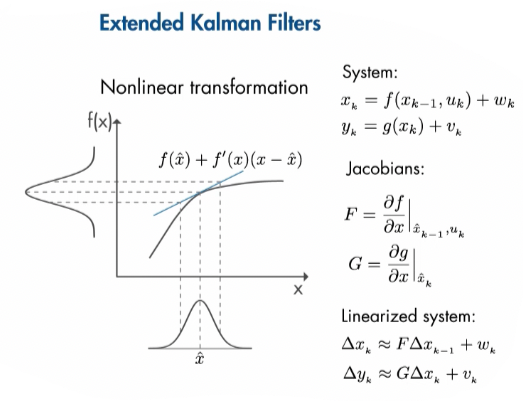
\includegraphics[width=8cm]{ekf3.png}
	\end{figure}
\end{frame}

\begin{frame}
	Drawbacks to Using Extended Kalman Filters (EKFs):
	\begin{itemize}
		\item  	It is difficult to calculate the Jacobians (if they need to be found analytically)
		\item There is a high computational cost (if the Jacobians can be found numerically)
		\item EKF only works on systems that have a differentiable model
		\item EKF is not optimal if the system is highly nonlinear
	\end{itemize}
%To address the issues with extended Kalman filters,  maybe  the unscented Kalman filter (UKF) or particle filter (PF) is useful.
For this case,  maybe  the unscented Kalman filter (UKF) or particle filter (PF) is useful.
	\begin{figure}
		\centering
		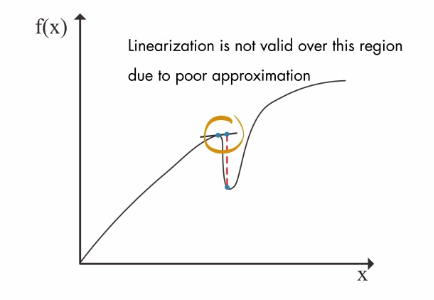
\includegraphics[width=5cm]{ukf2.png}
	\end{figure}
	UKF 
\end{frame}

\section{Example}
\subsection{UAV state estimation}

\begin{frame}
	\frametitle{Modeling}
	An example for implementing the Kalman filter is navigation where the vehicle state, position, and velocity are estimated by using sensor output from an inertial measurement unit (IMU) and a global navigation satellite system (GNSS) receiver. In this example, we consider only position and velocity, omitting attitude information. The three-dimensional position and velocity comprise the state vector:
	$$
	\boldsymbol{x}=\left[\boldsymbol{p}^T, \boldsymbol{v}^T\right]^T
	$$
	where $\boldsymbol{p}=\left[p_x, p_y, p_z\right]^T$ is the position vector and $\boldsymbol{v}=\left[v_x, v_y, v_{\mathbf{z}}\right]^T$ is the velocity vector whose elements are defined in $\mathrm{x}, \mathrm{y}, \mathrm{z}$ axes.
%	\begin{figure}
%		\centering
%		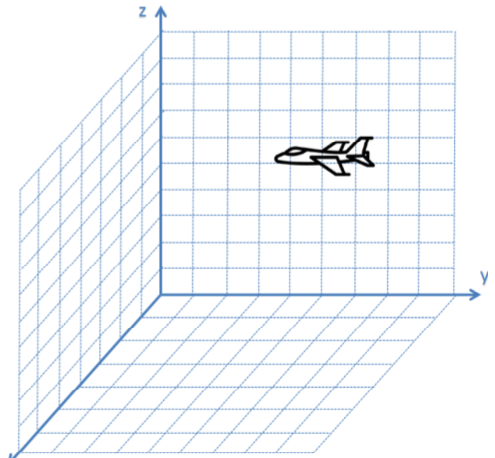
\includegraphics[width=11.5cm]{case1-1.png}
%	\end{figure}
\end{frame}

\begin{frame}
	The state in time $k$ can be predicted by the previous state in time $k-1$ as:
	$$
	\boldsymbol{x}_k=\left[\begin{array}{c}
		\boldsymbol{p}_k \\
		\boldsymbol{v}_k
	\end{array}\right]=\left[\begin{array}{r}
		\boldsymbol{p}_{k-1}+\boldsymbol{v}_{k-1} \Delta t+\frac{1}{2} \widetilde{\boldsymbol{a}}_{k-1} \Delta t^2 \\
		\boldsymbol{v}_{k-1}+\widetilde{\boldsymbol{a}}_{k-1} \Delta t
	\end{array}\right]
	$$
		\begin{figure}
				\centering
				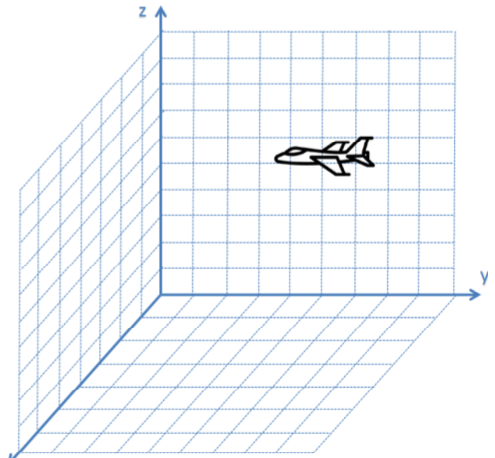
\includegraphics[width=6cm]{case1-1.png}
			\end{figure}
\end{frame}

\begin{frame}
	where $\tilde{\boldsymbol{a}}_{k-1}$ is the acceleration applied to the vehicle. The above equation can be rearranged as:
$$
\boldsymbol{x}_k=\left[\begin{array}{cc}
	I_{3 \times 3} & I_{3 \times 3} \Delta t \\
	0_{3 \times 3} & I_{3 \times 3}
\end{array}\right] \boldsymbol{x}_{k-1}+\left[\begin{array}{c}
	\frac{1}{2} I_{3 \times 3} \Delta t^2 \\
	I_{3 \times 3} \Delta t
\end{array}\right] \widetilde{\boldsymbol{a}}_{k-1}
$$

where $I_{3 \times 3}$ and $0_{3 \times 3}$ denote $3 \times 3$ identity and zero matrices, respectively. The process noise comes from the accelerometer output, $\boldsymbol{a}_{k-1}=\widetilde{\boldsymbol{a}}_{k-1}+\boldsymbol{e}_{k-1}$, where $\boldsymbol{e}_{k-1}$ denotes the noise of the accelerometer output. 
\end{frame}


\begin{frame}
    Suppose $\boldsymbol{e}_{k-1} \sim \mathcal{N}\left(0, I_{3 \times 3} \sigma_e^2\right)$. From the covariance relationship, $\operatorname{Cov}(A \boldsymbol{x})=A \Sigma A^T$ where $\operatorname{Cov}(\boldsymbol{x})=\Sigma$, we get the covariance matrix of the process noise as:
    $$
    Q=\left[\begin{array}{c}
    	\frac{1}{2} I_{3 \times 3} \Delta t^2 \\
    	I_{3 \times 3} \Delta t
    \end{array}\right] I_{3 \times 3} \sigma_e^2\left[\begin{array}{c}
    	\frac{1}{2} I_{3 \times 3} \Delta t^2 \\
    	I_{3 \times 3} \Delta t
    \end{array}\right]^T=\left[\begin{array}{cc}
    	\frac{1}{4} I_{3 \times 3} \Delta t^4 & 0_{3 \times 3} \\
    	0_{3 \times 3} & I_{3 \times 3} \Delta t^2
    \end{array}\right] \sigma_e^2
    $$
\end{frame}

\begin{frame}
	Now, we have the process model as:
	$$
	\boldsymbol{x}_k=F \boldsymbol{x}_{k-1}+B \boldsymbol{a}_{k-1}+\boldsymbol{w}_{k-1}
	$$
	where
	$$
	\begin{gathered}
		F=\left[\begin{array}{cc}
			I_{3 \times 3} & I_{3 \times 3} \Delta t \\
			0_{3 \times 3} & I_{3 \times 3}
		\end{array}\right] \\
		B=\left[\begin{array}{c}
			\frac{1}{2} I_{3 \times 3} \Delta t^2 \\
			I_{3 \times 3} \Delta t
		\end{array}\right] \\
		\boldsymbol{w}_{k-1} \sim \mathcal{N}(0, Q)
	\end{gathered}
	$$
	
\end{frame}

\begin{frame}
The GNSS receiver provides position and velocity measurements corrupted by measurement noise $\nu_k$ as:
$$
\mathbf{z}_k=\left[\begin{array}{c}
	\boldsymbol{p}_k \\
	\boldsymbol{v}_k
\end{array}\right]+\boldsymbol{\nu}_k
$$
It is straightforward to derive the measurement model as:
$$
\mathbf{z}_k=H \boldsymbol{x}_k+\nu_k
$$
where
$$
\begin{gathered}
	H=I_{6 \times 6} \\
	\nu_k \sim \mathcal{N}(0, R)
\end{gathered}
$$
\end{frame}



\begin{frame}
	\frametitle{Simulation settings}
	\begin{itemize}
		\item  In order to conduct a simulation to see how it works, let us consider $N=20$ time steps $(k=1,2,3, \ldots, N)$ with $\Delta t=1$. It is recommended to generate a time history of true state, or a true trajectory, first. 
		\item The most convenient way is to generate the series of true accelerations over time and integrate them to get true velocity and position.
		\item  In this example, the true acceleration is set to zero and the vehicle is moving with a constant velocity, $v_k=[5,5,0]^T$ for all $k=1,2,3, \ldots, N$, from the initial position, $\boldsymbol{p}_0=[0,0,0]$. 
	
	\end{itemize}
\end{frame}

\begin{frame}
	\frametitle{Simulation settings}
	\begin{itemize}
		\item  We need to generate noise of acceleration output and GNSS measurements for every time step. Suppose the acceleration output, GNSS position, and GNSS velocity are corrupted with noise with variances of $0.3^2, 3^2$, and $0.03^2$, respectively. 
		\item The process noise covariance matrix, $Q$, and measurement noise covariance matrix, $R$, can be constructed following the real noise statistics described above to get the best performance. However, have in mind that in real applications, we do not know the real statistics of the noises and the noises are often not Gaussian. Common practice is to conservatively set $Q$ and $R$ slightly larger than the expected values to get robustness.
		
	\end{itemize}
\end{frame}


\begin{frame}
Let us start filtering with the initial guesses
$$
\begin{aligned}
	& \hat{\boldsymbol{x}}_0^{+}=[2,-2,0,5,5.1,0.1]^T \\
	& P_0^{+}=\left[\begin{array}{cc}
		I_{3 \times 3} 4^2 & 0_{3 \times 3} \\
		0_{3 \times 3} & I_{3 \times 3} 0.4^2
	\end{array}\right]
\end{aligned}
$$
and noise covariance matrices
$$
\begin{gathered}
	Q=\left[\begin{array}{cc}
		\frac{1}{4} I_{3 \times 3} \Delta t^4 & 0_{3 \times 3} \\
		0_{3 \times 3} & I_{3 \times 3} \Delta t^2
	\end{array}\right] 0.3^2 \\
	R=\left[\begin{array}{cc}
		I_{3 \times 3} 3^2 & 0_{3 \times 3} \\
		0_{3 \times 3} & I_{3 \times 3} 0.03^2
	\end{array}\right]
\end{gathered}
$$
where Q and R are constant for every time step. The more uncertain your initial guess for the state is, the larger the initial error covariance should be.
\end{frame}


\begin{frame}
	\frametitle{Result}
	Actual and estimated standard deviation for x-axis estimate errors: 
	\begin{figure}
		\centering
		\includegraphics[width=7cm]{standard_deviation.png}
	\end{figure}
\end{frame}

\begin{frame}
	\frametitle{Hardware test configuration}
	\begin{figure}
		\centering
		\includegraphics[width=8.5cm]{test.png}
	\end{figure}
\end{frame}
\begin{frame}
	\frametitle{Source code}

	\begin{itemize}
		\item \href{ https://github.com/PX4/PX4-Autopilot}{\color{blue}{\underline{PX4}}}: PX4 is the Professional Autopilot. Developed by world-class developers from industry and academia, and supported by an active world wide community, it powers all kinds of vehicles from racing and cargo drones through to ground vehicles and submersibles.
		
		\item \href{https://github.com/mengchaoheng/PX4-ECL}{\color{blue}{\underline{ECL}}}: Very lightweight Estimation and Control Library. Added support for running offline by Meng ChaoHeng.
	\end{itemize}
\end{frame}

\end{document}

